\section{Results}
\label{section:results}
Spiking neural networks have notoriously been a challenge to train. Reinforcement learning on the other hand, is highly sensitive to factors such as hyperparameter tuning. The combination of SNNs trained with an RL framework therefore showed a challenging task. Therefore, we start by comparing the training patterns of SNNs compared to ANN. Next, an analysis is carried out on the complexity of both the neuromorphic and conventional solution, using NeuroBench. Lastly, it is analyzed how the introduction of noise on the sensor inputs affect the performance of the algorithm. This reflects the behavior of the trained agents in a more realistic setting. 
\\
\subsection{Training}
For the control of the CartPole, multiple policies were trained, divided in two architecture types. First, models with a single hidden layer were trained, then, models using two hidden layers were trained. Of both policy types, at least one conventional and one neuromorphic solution was trained. Due to the simplicity of this task, it can be observed that all models are able to achieve a reasonable performance. As expected, for both the deeper model as the model with only one hidden layer, the neuromorphic solution converges slower. This can partly be explained by the way the surrogate gradient, used during backpropagation, works. Where in a conventional neural network, virtually all weights contribute to the output at each timestep, for spiking neural networks this is not the case. Neurons for which the potential at a timestep is lower than the threshold, will not spike. Therefore, for this instant, there is no backpropagation gradient past this neuron.

\autoref{fig:trainging_1layer} shows the reward obtained by the agent after every episode of the training cycle. Allowing the network to train the amount of leakage of the neurons leads to fast convergence and relatively high performance. However, upon further inspection of the trained model, it can be seen that the model learns to have complete leakage at every timestep ($\beta=0$ in Equation (1)). This thus corresponds to an ANN with a Heaviside threshold function which goes from zero to one at the threshold value. Therefore, no temporal dynamics are learned. In a subsequent training cycle, the leak, $\beta$ was fixed to a value of 0.65. Initially this leads to faster training, as less parameters need to be learned. However, the training is less stable and the final model is not able to reach a competitive performance to the other trained models. 

\begin{figure}[h]
    \centering
    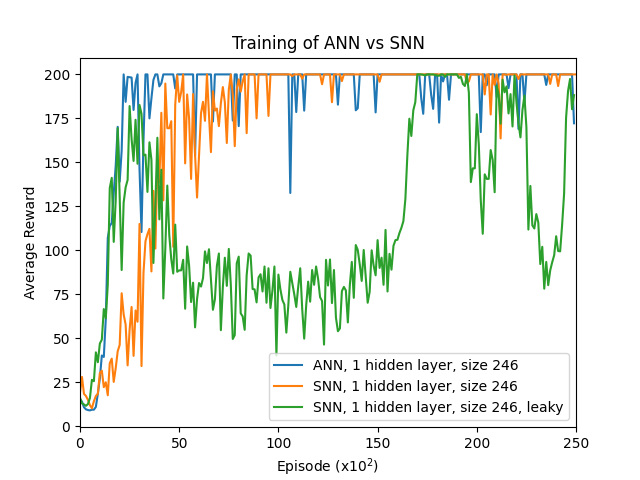
\includegraphics[width = .45\textwidth]{Figures/training_3models.png}
    \caption{Training of an ANN and SNN with one hidden layer of size 246. The first SNN learns to reduce $\beta$ to zero. The second SNN has a fixed leak, $\beta=0.65$.}
    \label{fig:trainging_1layer}
\end{figure}

Next, the deeper models were trained, presented on \autoref{fig:trainging_two_layers}. These showed a slower convergence, due to the increased effect of the vanishing gradients. However, the training showed more stable behavior. Interestingly, it was found that the training of SNN showed to be easier when the weight of the entropy loss was increased, encouraging random actions.
\begin{figure}[h]
    \centering
    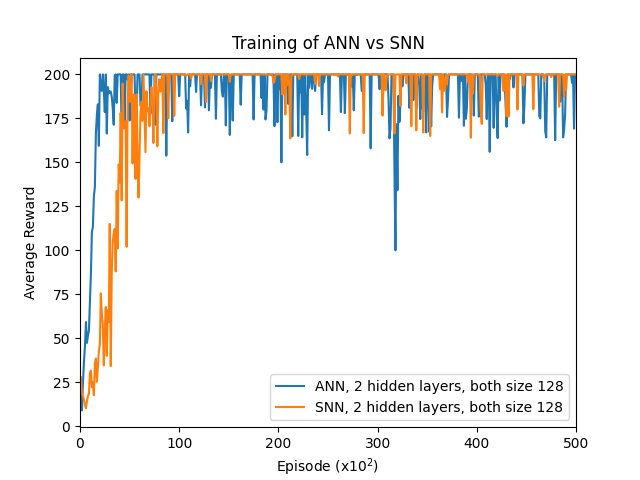
\includegraphics[width = .45\textwidth]{Figures/Training_SNNANN2layers.png}
    \caption{Training of an ANN and SNN with two hidden layers of size 128. The SNN has a leak of $\beta=1.$ $\beta=0.95$ for the first and second spiking layer respectively.}
    \label{fig:trainging_two_layers}
\end{figure}
For the hyperparameters used, the public GitHub repository can be consulted \footnote{\url{https://github.com/korneelf1/SpikingA2C}}.
% \begin{figure}
%     \centering
%     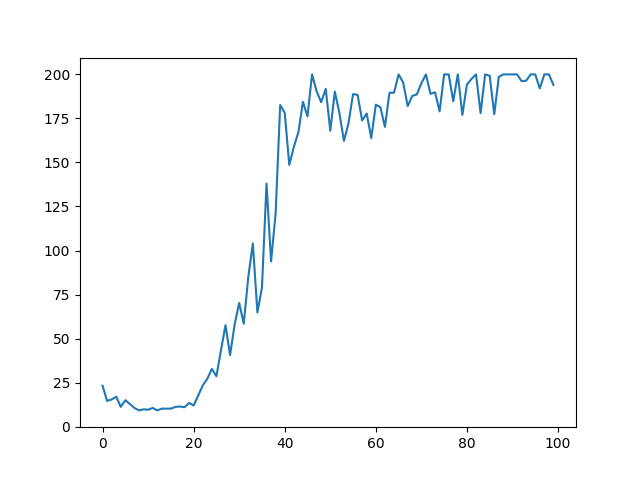
\includegraphics[width = .45\textwidth]{Figures/ANN44_20HZ.png}
%     \caption{One small hidden layer}
%     \label{fig:enter-label}
% \end{figure}

\subsection{Performance and computational complexity}
Using NeuroBench \footnote{\url{https://neurobench.ai}}, a fair comparison can be made between the trained models. The benchmark provides performance and complexity metrics. For more information on the metrics, the article can be consulted. While NeuroBench does not officially support the benchmarking of closed-loop systems yet, an initial effort towards benchmarking these systems is publicly available on the GitHub repository \footnote{\url{https://github.com/NeuroBench/neurobench}}. The benchmark starts 1000 interactions with the environment, each limited to a maximum of 10000 steps and monitors the model performance and complexity. Performance for this task is defined as the average obtained reward and the standard deviation. Furthermore, inspired by A2Perf \footnote{\url{https://github.com/Farama-Foundation/A2Perf#rlperf-benchmark-for-autonomous-agents}}, the risk is computed as well. This risk is defined as the average of the $5\%$ lowest scoring interactions. The complexity metrics on the other hand, include the footprint, model frequency (which is defined to be 20Hz for all models), the connection sparsity, activation sparsity and the synaptic operations required per prediction. 

First, the shallow models, having a hidden layer of size 246 are analysed. \autoref{tab:in246out_results_ANN} presents the results for the ANN, while \autoref{tab:in246out_results_SNN} presents the results for the SNN without temporal dynamics, as well as the SNN with a fixed leak of $\beta=0.65$.
\begin{table}[h]
\centering
\renewcommand{\arraystretch}{1.5}
\begin{tabular}{c|c} \thickhline
 Baseline & ANN\\ \hline
 Reward (mean $\pm$ std) & 1744 $\pm$ 1385 \\
 Risk & 190 \\ \hline
 Footprint (bytes) & $7.9 \times 10^3$ \\
 Activation Sparsity & 0.0 \\
 SynOps Dense & $1.7 \times 10^{3}$ \\
 SynOps Eff\_MACs & $1.5 \times 10^{3}$ \\
 SynOps Eff\_ACs & 0 \\ \thickhline
\end{tabular}
\caption{NeuroBench results for the single layer ANN controlling the CartPole task.}
\label{tab:in246out_results_ANN}
\end{table}
\begin{table}[h]
\centering
\renewcommand{\arraystretch}{1.5}
\begin{tabular}{c|cc} \thickhline
 Baseline  & SNN& SNN, leaky\\ \hline
 Reward (mean $\pm$ std)  & 1620$\pm$1600& 232$\pm$65 \\
 Risk  & 148& 152\\ \hline
 Footprint (bytes)  & $7.9 \times 10^3$& $7.9 \times 10^3$ \\
 Activation Sparsity & 0.68& 0.92\\
 SynOps Dense  & $1.7 \times 10^{3}$ & $1.7 \times 10^{3}$\\
 SynOps Eff\_MACs & $0.9\times 10^{3}$ &$0.9\times 10^{3}$\\
 SynOps Eff\_ACs & 238 &59\\ \thickhline
\end{tabular}
\caption{NeuroBench results for the single layer SNNs controlling the CartPole task.}
\label{tab:in246out_results_SNN}
\end{table}\\
As expected the ANN outperforms the SNN variants when looking at the reward characteristics. The well established training techniques and the reinforcement learning algorithm that was originally made for ANN, shows effective training of ANN for the CartPole task. Comparing the two SNN models (\autoref{fig:trainging_1layer}, it shows that the first one, which did not learn temporal dynamics, is able to achieve a significantly higher mean reward than the leaking model. However, when looking at the standard deviation and risks of both models, the leaky SNN tends to be more predictable and even less risky.
\\
Next, the differences in the results of the complexity metrics display where SNN models shine compared to the better performing ANN equivalent. Thanks to the spiking nature of SNN, layers after a spiking layer only require accumulates (AC) rather than multiply accumulates (MACs). Where an AC consists of one operation, the addition, the MAC requires a multiplication and an addition. The multiply operation is more energy demanding than the addition. Therefore, computing an AC is much less intensive. Furthermore, thanks to the sparsity in the spiking models, the effective operations required, is significantly reduced. These effective operations are defined as operations where non-zero inputs are multiplied by non-zero weights. Specialized hardware could make use of these characteristics and reduce the computational effort required for these operations. Furthermore, it can be seen that the encoding layer, which is a linear layer connecting the continuous input to the first spiking layer, accounts for the largest number of operations in the spiking model. Therefore, more efficient spiking encoders could significantly reduce the complexity of the model.
\\
\autoref{tab:in128x2out_results} shows the results on the deeper models tested through NeuroBench. It can be seen that the deeper model significantly increases the required footprint and number of dense operations. However, the number of MACs for the SNN, representing the encoding, has decreased when comparing with the single layer models with a larger hidden layer. The performance of the models is observed to decrease significantly, due to the increased effect of dead and saturated neurons in deeper models. This leads to a significant reduction in the performance of the $5\%$ scoring interactions, reflected by the risk metric.
\begin{table}[ht]
\centering
\renewcommand{\arraystretch}{1.5}
\begin{tabular}{c|cc} \thickhline
 Baseline & ANN, 2 layers& SNN, 2 layers\\ \hline
 Reward (mean $\pm$ std) & 360 $\pm$ 116 & 220$\pm$139 \\
 Risk & 97 & 27\\ \hline
 Footprint (bytes) & $70 \times 10^3$ & $70 \times 10^3$ \\
 Activation Sparsity & 0.0 & 0.82\\
 SynOps Dense & $17 \times 10^{3}$ & $17 \times 10^{3}$ \\
 SynOps Eff\_MACs & $10 \times 10^{3}$ & $0.5\times 10^{3}$ \\
 SynOps Eff\_ACs & 0 & $4.2 \times 10^{3}$\\ \thickhline
\end{tabular}
\caption{NeuroBench results for the double layer models controlling the CartPole task.}
\label{tab:in128x2out_results}
\end{table}

\subsection{Pruning}
When training spiking neural networks using surrogate gradients, two undesired effects can occur. Dead neurons and saturated neurons. This is caused by the input current being very low or very high, leading to a non-spiking or continuously spiking neuron respectively. The gradient of the surrogate function is always zero, countering the flow of gradients through the net. While this is a highly undesired behavior during training, it does leave the opportunity to get rid of these neurons. For both the single layer spiking models, these neurons were removed. Firstly, the dead neurons and their connecting synapses are completely removed. Secondly, the synapses for which the post-synaptic neuron is saturated, are removed. For the synapses for which the pre-synaptic neuron is saturated, the synaptic weight is added as a bias to the post-synaptic neuron. \\
To identify these neurons, the model interacts with the environment 1000 times, during which the spiking activity for each neuron is registered. Neurons with $0\%$ or $100\%$ spiking activity are removed as described above. This theoretically should not affect the performance, however due to neurons that have near $0\%$ or $100\%$ spiking activity, some neurons are wrongfully classified as dead or saturated. This effect can be reduced by increasing the number of interactions with the environment. This led to impressive results in the consequent NeuroBench tests. Running the pruning algorithm on the first single layer SNN, with a $\beta$ of 0, we were able to remove 235 neurons, leaving us with a hidden layer of only 11 neurons. For the second SNN, with  a $\beta$ of 0.65, we were able to remove 225 neurons, which leads to a hidden layer size of 21. This is reflected in \autoref{tab:inprunedout_results}. Note that for this NeuroBench run, the critic head was removed, as this does not add any functionality during the inference of the agent. Including this head would lead to an increase in ACs of at most 11 and 21 for the pruned SNN and the pruned leaky SNN respectively.
\\
These pruned models show the pruning possibilities when using spiking neural networks trained with A2C. While performance does not degrade significantly, the footprint and operations required reduce roughly with a factor 20 and 25 respectively. While the largest computational effort still is attributed to the encoding layer (reflected in the effective MAC metric), the reduction in complexity using non-neuromorphic hardware is still promising, now only requiring 66 dense operations, versus the 1700 operations required for the previous model. 
\begin{table}[ht]
\centering
\renewcommand{\arraystretch}{1.5}
\begin{tabular}{c|cc} \thickhline
 Baseline & SNN pruned & SNN, leaky pruned \\ \hline
 Reward (mean $\pm$ std) & 1570 $\pm$ 1480 & 200$\pm$64  \\
 Risk & 140 & 73 \\ \hline
 Footprint (bytes) & 360 & 640\\
 Activation Sparsity & 0.49 & 0.65 \\
 SynOps Dense & 66 & 126 \\
 SynOps Eff\_MACs & 44 & 84 \\
 SynOps Eff\_ACs & 12 & 16 \\ \thickhline
\end{tabular}
\caption{NeuroBench results for the pruned single layer SNNs controlling the CartPole task.}
\label{tab:inprunedout_results}
\end{table}

After analyzing the great reduction in complexity after the pruning of the SNN, a model with the same architecture, replacing the spiking neurons with ReLU activation functions, was trained for the same number of episodes as the original SNN. Training this network with a single hidden layer of 11 neurons showed a significant decrease in performance comparing to the original ANN and even compared to the pruned SNNs. Where the pruned SNNs were able to have a relatively small decrease in average performance and a reasonable risk, the ANN's average performance degraded significantly with a risk that may be unacceptable in some circumstances. Again, for this analysis, the critic head was removed.
\begin{table}[ht]
\centering
\renewcommand{\arraystretch}{1.5}
\begin{tabular}{c|c} \thickhline
 Baseline & ANN 11 neurons  \\ \hline
 Reward (mean $\pm$ std) & 263 $\pm$ 114 \\
 Risk & 42\\ \hline
 Footprint (bytes) & 360\\
 Activation Sparsity & 0.0 \\
 SynOps Dense & 66  \\
 SynOps Eff\_MACs & 66\\
 SynOps Eff\_ACs & 0 \\ \thickhline
\end{tabular}
\caption{NeuroBench results for the ANN with 11 hidden neurons controlling the CartPole task.}
\label{tab:inprunedout_results}
\end{table}
\\
For the deeper models, it is hypothesised that similar results can be obtained. However, due to time restrictions, the pruning of deeper SNN is left as future work.

\subsection{Noise robustness}
When deploying controllers in the real world, the observations will be affected by noise. The noise robustness of controllers can therefore be a significant factor in the decision on what algorithm is suitable for its usecase. This subsection therefore attempts to characterize the behaviour of all aforementioned models under noise.\\
As explained in the previous sections, allowing the leakage to be trained causes the neuron to disregard temporal dynamics completely. Constraining the leakage to non-zero numbers, necessitates the model to learn the temporal dynamics of the system. This leads to longer and more difficult training for the SNN. On the other side, it is often hypothesized that the temporal spiking nature of SNN could lead to noise robustness. Therefore, we conducted an experiment to analyze the performance of the trained models after injecting noise, to more closely simulate real-world imperfections. \\
Experiments were carried out to asses the noise robustness of the trained models. For a range of a gain of 0 to 1 with a step size of 0.015, each model was evaluated 250 times, with a maximum interaction time of 1000. These parameters were chosen to sufficiently represent the behaviour under noise, while reducing the computational resources needed to generate the results. 
\\
\autoref{fig:SNNvsANN_Noise} displays the results of the previously described experiment. It can be seen that the models which exploit the leakage of the neurons tend to be more noise robust. At a noise level of roughly 0.15, these models outperform their non leaking counterparts. The non leaking models tend to show a high degradation of performance when noise is injected. 

\begin{figure}[h]
    \centering
    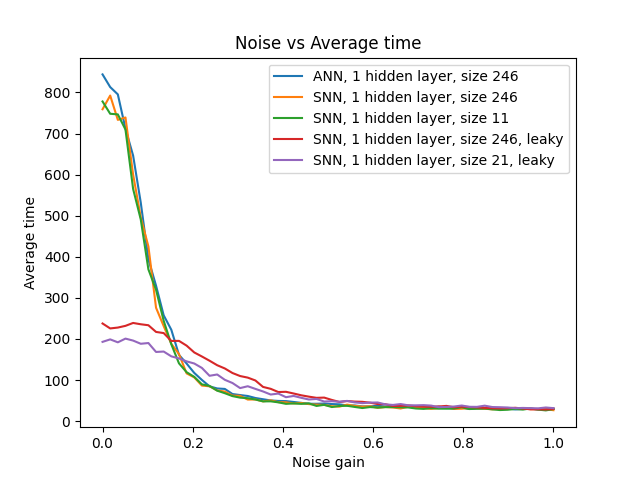
\includegraphics[width = .45\textwidth]{Figures/Noise_Robustness_5Models.png}
    \caption{Noise robustness analysis of the previously described single layer models.}
    \label{fig:SNNvsANN_Noise}
\end{figure}


Performing the same analysis for the deeper models leads to similar results, as shown on \autoref{fig:SNNvsANN_Noise_2layers}. At an injected noise with gain of $0.04$, the performance of the SNN surpasses the ANN.

\begin{figure}[h]
    \centering
    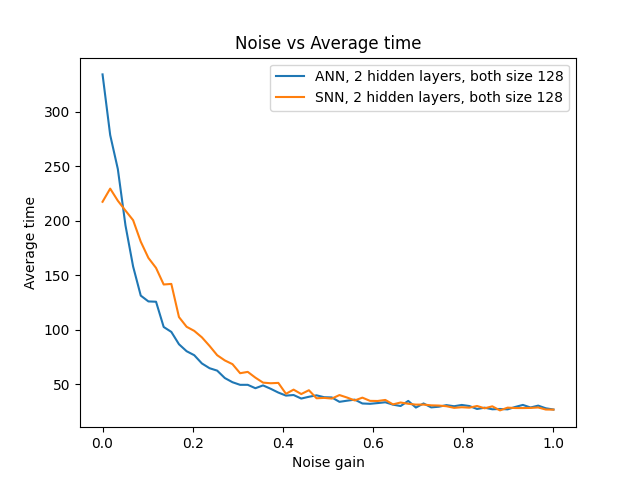
\includegraphics[width = .45\textwidth]{Figures/Noise_Robustness_2layer_models.png}
    \caption{Noise robustness analysis of the previously described double layer models.}
    \label{fig:SNNvsANN_Noise_2layers}
\end{figure}
% This unexpected behavior repeated with all of the leaking SNN models trained. The noise level for peak of performance varied with the amount of leakage present in the neurons. A further experiment lead to injecting noise in the observations during training. This lead to a marginally improved performance, while increasing the training time. It also lead to a reduced noise level for peak performance of the SNN (\autoref{fig:SNN_TrainedwithNoisevsANN_Noise}, reducing the range for which ANN are significantly better. Further work should investigate the effect of the noise injection on performance of SNN and ANN to enable a reasoned choice of algorithm for specific functions. 

% \begin{figure}
%     \centering
%     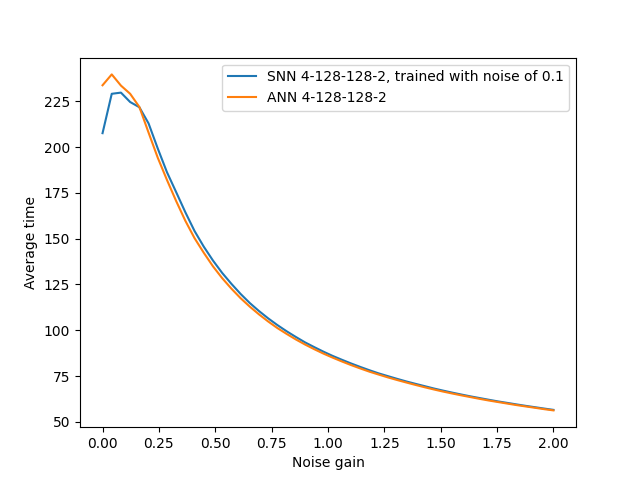
\includegraphics[width = .45\textwidth]{Figures/Trained_with_Noise.png}
%     \caption{Noise robustness of an SNN with leakage, trained with an injected noise level of 0.1 and an ANN.}
%     \label{fig:SNN_TrainedwithNoisevsANN_Noise}
% \end{figure}\textbf{}

